\PassOptionsToPackage{table}{xcolor}   % house style: striped tables (extras.tex)
%%%%%%%%%%%%%%%%%%%%%%%%%%%%%%%%%%%%%%%%%
% Macro Regime–Based Asset Rotation
% Two-column academic journal style
% Modeled after the uploaded LaTeX article template
%%%%%%%%%%%%%%%%%%%%%%%%%%%%%%%%%%%%%%%%%

\documentclass[10pt, a4paper, twocolumn]{article}

% ─── Packages ───────────────────────────────────────
\usepackage[utf8]{inputenc}
\usepackage[T1]{fontenc}
\usepackage{mathpazo}                       % Palatino font (matches template)
\usepackage{microtype}                      % Better typography
\usepackage[english]{babel}
\usepackage{amsmath,amssymb,amsfonts}
\usepackage{graphicx}
\usepackage{booktabs}
\usepackage{tabularx}
\usepackage{float}
\usepackage{caption}
\usepackage{subcaption}
\usepackage[colorlinks=true,linkcolor=blue,citecolor=blue,urlcolor=blue]{hyperref}
\usepackage[numbers,sort&compress]{natbib}
\usepackage{fancyhdr}
\usepackage{geometry}
\usepackage{enumitem}
\usepackage{xcolor}
\usepackage{titlesec}
\usepackage{abstract}
\usepackage{etoolbox}
\usepackage{multirow}
\usepackage{array}
\usepackage{makecell}

% ─── Page geometry (matches template) ──────────────
\geometry{
  top=2.0cm,
  bottom=2.0cm,
  left=1.8cm,
  right=1.8cm,
  columnsep=0.8cm
}

% ─── Header / footer (journal style like template) ─
\pagestyle{fancy}
\fancyhf{}
\renewcommand{\headrulewidth}{0.4pt}
\fancyhead[L]{\small\textit{Delta-Hedged Gamma on SPY and QQQ: A Research Design}}
\fancyhead[R]{\small\textit{QUANTT Research}}
\fancyfoot[L]{\small\textit{Queen's University Algorithmic \& Network Trading Team (2026)}}
\fancyfoot[R]{\small\thepage}

% ─── Section formatting (centered, matches template) ──
\titleformat{\section}
  {\large\bfseries\centering}{\thesection.}{0.5em}{}
\titleformat{\subsection}
  {\normalsize\bfseries}{\thesubsection}{0.5em}{}
\titleformat{\subsubsection}
  {\normalsize\bfseries\itshape}{\thesubsubsection}{0.5em}{}

% ─── Abstract formatting ─────────────────────────────
\renewcommand{\abstractnamefont}{\normalfont\bfseries}
\renewcommand{\abstracttextfont}{\normalfont\small\itshape}

% ─── Float spacing (tighten gaps around tables/figures) ──
\setlength{\textfloatsep}{8pt plus 2pt minus 2pt}
\setlength{\intextsep}{8pt plus 2pt minus 2pt}
\setlength{\floatsep}{8pt plus 2pt minus 2pt}
\setlength{\abovecaptionskip}{4pt}
\setlength{\belowcaptionskip}{2pt}

% ─── Custom commands ──────────────────────────────────
\newcommand{\shratio}{\text{Sharpe}}
\newcommand{\regime}[1]{\textsc{#1}}

%═══════════════════════════════════════════════════════
% ─── House additions (load right after preamble.tex, before \begin{document}) ───
% Needs \PassOptionsToPackage{table}{xcolor} as the FIRST line of the .tex file (before \documentclass).
% Navy accent on headings, captions and table rules; striped tables; a key-findings box.
\usepackage{colortbl}
\usepackage[most]{tcolorbox}
\definecolor{qnavy}{HTML}{1B365D}
\definecolor{qblue}{HTML}{4A7AB5}
\definecolor{qstripe}{HTML}{F2F5FA}
\definecolor{qbox}{HTML}{EEF2F8}

\titleformat{\section}{\large\bfseries\centering\color{qnavy}}{\thesection.}{0.5em}{}
\titleformat{\subsection}{\normalsize\bfseries\color{qnavy}}{\thesubsection}{0.5em}{}
\titleformat{\subsubsection}{\normalsize\bfseries\itshape\color{qnavy}}{\thesubsubsection}{0.5em}{}

\captionsetup{font=small, labelfont={bf,color=qnavy}, labelsep=period}
\hypersetup{linkcolor=qblue, citecolor=qblue, urlcolor=qblue}

% Booktabs rules in navy; zebra rows with \qstripes before the tabular (inside the table float).
\makeatletter
\renewcommand{\toprule}{\arrayrulecolor{qnavy}\specialrule{\heavyrulewidth}{\abovetopsep}{\belowrulesep}\arrayrulecolor{black}}
\renewcommand{\bottomrule}{\arrayrulecolor{qnavy}\specialrule{\heavyrulewidth}{\aboverulesep}{\belowbottomsep}\arrayrulecolor{black}}
\makeatother
\newcommand{\qstripes}{\rowcolors{2}{qstripe}{white}}
\newcommand{\qhead}[1]{\textbf{\color{qnavy}#1}}

% Key findings: full width (put it inside the \twocolumn[{...}] title block after the abstract,
% or in a figure*). Usage: \begin{keyfindings} \item ... \end{keyfindings}
\newenvironment{keyfindings}
  {\begin{tcolorbox}[enhanced, colback=qbox, colframe=qnavy, boxrule=0pt, leftrule=2.5pt,
     arc=0pt, left=6pt, right=6pt, top=4pt, bottom=4pt, fontupper=\small,
     title={\small\bfseries Key findings}, coltitle=qnavy, colbacktitle=qbox, attach title to upper={\par\vspace{2pt}}]
   \begin{itemize}[nosep, leftmargin=*, label={\color{qnavy}\textbullet}]}
  {\end{itemize}\end{tcolorbox}}

% Source line under a figure or table: \qsource{CRSP via WRDS; author's calculations.}
\newcommand{\qsource}[1]{\par\vspace{1pt}{\footnotesize\color{black!60}\textit{Source:} #1}\par}
\begin{document}
\raggedbottom
\newcolumntype{L}[1]{>{\raggedright\arraybackslash}p{#1}}
\newcolumntype{Y}{>{\raggedright\arraybackslash}X}
\makeatletter
\newcommand{\qneed}[1]{\par\penalty-100\begingroup\setlength{\dimen@}{#1}\dimen@ii\pagegoal\advance\dimen@ii-\pagetotal\ifdim\dimen@>\dimen@ii\ifdim\dimen@ii>\z@\vfil\fi\break\fi\endgroup}
\makeatother
\renewcommand{\dbltopfraction}{0.9}
\setcounter{dbltopnumber}{2}
\renewcommand{\topfraction}{0.85}

% ─── Title block (full-width, matches template style) ─
\twocolumn[{%
\begin{center}
{\LARGE\bfseries Delta-Hedged Gamma on SPY and QQQ Options:\\
Evidence, Data and a Proposed Test\par}
\vspace{0.8em}
{\large Simon Jarvis\par}
\vspace{0.4em}
{\normalsize
QUANTT --- Queen's University Algorithmic \& Network Trading Team\\
\vspace{0.3em}
}
\vspace{0.5em}

% ─── Abstract (boxed, italic, matching template) ──────
\begin{minipage}{0.92\textwidth}
\rule{\linewidth}{0.4pt}
\vspace{0.3em}
\textbf{Abstract}\\[0.3em]
\small\itshape
This paper is a research design, not a backtest. It asks whether a delta-hedged options book on SPY and QQQ, the exchange-traded funds that track the S\&P~500 and the Nasdaq-100, can earn the variance risk premium, and how it should be sized and hedged. No backtest of our own has been run and no code has been written: every return figure quoted here comes from the published literature, mostly on S\&P~500 index (SPX) options, gross of costs at mid quotes. That literature finds that delta-hedged index options lose money for the buyer on average; over 1996--2003 the 30-day synthetic variance swap rate on SPX averaged 24.4 volatility points against 18.8 realised. One recent, unrefereed working paper finds that the risk-adjusted part of the premium has been about zero since around 2010, so what remains looks mainly like payment for crash risk. The slope of the VIX term structure is the best-supported signal for scaling a short-volatility position, and we found no verified evidence of a state in which a long delta-hedged position has positive expected value. We hold twelve years of SPY and QQQ option trade prints but no quotes, open interest or implied volatilities, and the archive has known gaps, including every month-end trading day. We propose a first test on 2016 to July 2026: a 30-day SPY iron fly, delta-hedged with shares under three hedging rules, sized by the term-structure slope, with implied volatilities rebuilt from trade prints and checked against a live chain, and judged on tail losses against holding equity beta.
\vspace{0.3em}
\rule{\linewidth}{0.4pt}
\end{minipage}

\vspace{0.6em}
\begin{minipage}{0.92\textwidth}
\begin{keyfindings}
\item Buyers of delta-hedged index options have lost on average: from January 1996 to February 2003 the 30-day SPX synthetic variance swap rate averaged 24.4 volatility points against 18.8 realised.
\item The risk-adjusted edge has faded: since about 2010 the CAPM alpha of delta-hedged SPX options is about zero, and the information ratio of long 5\% out-of-the-money puts moved from about $-0.6$ to $0.09$ (one unrefereed study).
\item The VIX term-structure slope is the best-supported sizing signal. No study we checked finds a state in which long delta-hedged gamma pays, and none uses data after 2022 or reports results net of costs.
\item Our archive holds 1.347 billion SPY and 585 million QQQ option trades from June 2014 to July 2026, but no quotes, implied volatilities or open interest, and every month-end trading day is missing.
\item SPY option trades per day rose from about 67,000 in 2017 to about 1.07 million in 2025; on a July 2026 sample day 70\% were in same-day expiries.
\item The proposed first test, not yet run, is a 30-day SPY iron fly from 2016 to July 2026, delta-hedged under three rules and judged on tail losses against holding equity beta.
\end{keyfindings}
\end{minipage}

\vspace{0.3em}
{\footnotesize \textbf{Date:} November 2026. \textbf{Status:} research design; the proposed backtest has not been run.}
\end{center}
\vspace{1em}
}]

%═══════════════════════════════════════════════════════
\section{Introduction}
\label{sec:intro}

A trader who sells an option and hedges its exposure to the direction of the underlying is left holding a bet on the size of future price moves. If the volatility implied by the option's price is higher than the volatility the underlying then realises, the seller profits. The average gap between implied and subsequently realised variance is the variance risk premium, and a long literature, almost all of it on S\&P~500 index options, finds that it has historically favoured sellers.

This paper asks whether a small systematic desk could run a delta-hedged options book on SPY and QQQ options with the data it holds and the broker it uses, Alpaca. It has three parts: a structured review of the literature on the premium, on signals for sizing it, on dealer gamma and on hedging under costs; a check, made on 29~September 2026, of what our option archive and Alpaca's API can and cannot support; and a backtest design with the rules by which its result will be judged.

\emph{No backtest of our own has been run, and no code has been written.} Every return, information ratio and regression coefficient below is a figure reported by a cited study, almost always on SPX or S\&P~500 futures options rather than on SPY or QQQ, gross of costs and at mid quotes. None of it is a result of ours.

The review leads to a specific proposal: a short delta-hedged gamma position on SPY, sized between full and flat by volatility regime, with a long-gamma position kept only as a comparison case, because we found no verified evidence of a regime in which it pays. The broker does not allow naked short straddles, so the short position must be a defined-risk four-leg structure, and each delta hedge is a separate share order. Section~\ref{sec:background} sets out the mechanics, Section~\ref{sec:lit} the literature, Section~\ref{sec:data} the data, Section~\ref{sec:design} the test, and Section~\ref{sec:open} the open questions.

%═══════════════════════════════════════════════════════
\qneed{7\baselineskip}
\section{Background}
\label{sec:background}

\subsection{Gamma, delta hedging and the premium}

An option's delta, $\Delta=\partial V/\partial S$, is the change in its value for a small change in the underlying price $S$; its gamma, $\Gamma=\partial^2 V/\partial S^2$, is the rate at which delta changes. A delta-hedged position holds an offsetting number of shares, so small price moves leave its value unchanged to first order and what remains is exposure to the size of moves. Long options are long gamma and gain when the underlying moves more than the implied volatility priced in; short options gain when it moves less. The standard per-period decomposition is
\begin{equation}
\mathrm{d}\Pi \approx \tfrac{1}{2}\,\Gamma\,S^{2}\left(\sigma_R^{2}-\sigma_I^{2}\right)\mathrm{d}t \;+\; \text{vega and cost terms},
\label{eq:pnl}
\end{equation}
with $\sigma_R$ realised and $\sigma_I$ implied volatility. This is the standard textbook decomposition.

A variance swap pays realised variance over its life minus a fixed strike set at the start; a \emph{synthetic} variance swap rate is that strike computed from a strip of option prices, so it measures implied variance \cite{carrwu2009}. Ahmad and Wilmott \cite{ahmad2005} note that a delta-hedged trade involves three volatilities: the implied volatility paid, the volatility actually realised, and the volatility used to compute the hedge ratio. The last is a design choice separate from the view on implied against realised volatility; practitioner summaries describe hedging at implied volatility as giving a smoother but path-dependent profit, and hedging at the forecast realised volatility as locking in the expected profit along a noisier path.

\subsection{SPX against SPY and QQQ}

Nearly all the evidence below is on SPX or S\&P~500 futures options, which are European-style and settle in cash. SPY and QQQ options are American-style, written on funds that pay dividends, settle in shares and carry heavy retail order flow. Early exercise and dividends therefore enter the price of every SPY and QQQ option, and SPX results cannot be carried over untested. Both SPY and QQQ now list options that expire every trading day (zero days to expiry, or 0DTE).

\subsection{Short gamma with defined risk}

A long straddle buys an at-the-money call and put with the same strike and expiry; selling the pair is a short straddle. An \emph{iron fly} is a short straddle with a long out-of-the-money put and call added as ``wings''; an \emph{iron condor} sells an out-of-the-money put and call and buys wings further out. Both have four legs and a loss capped by the wings, which cost part of the premium.

\subsection{Dealer gamma}

The aggregate gamma of option market makers (dealers), often called gamma exposure or GEX, is used to describe whether their hedging tends to go with price moves (dealers net short gamma) or against them (net long). Dealer positions are not observed, so the standard academic proxy assumes that dealers are long every call and short every put outstanding \cite{baltussen2021}:
\begin{equation}
\mathrm{NGE}_t = \frac{1}{\mathrm{MV}_t}\sum_i s_i\,\Gamma_{i,t}\,\mathrm{OI}_{i,t}\times 100\times S_t ,
\label{eq:gex}
\end{equation}
with $s_i=+1$ for calls and $-1$ for puts, $\mathrm{OI}$ the open interest in contracts, $S_t$ the index level and $\mathrm{MV}_t$ the index market value. It needs open interest by strike, which a trade-print archive does not contain.

%═══════════════════════════════════════════════════════
\section{What the Literature Finds}
\label{sec:lit}

\subsection{How the review was done}

The review, completed on 29~September 2026, covered five topics: the variance risk premium and delta-hedged returns; hedging rules under transaction costs; forecasting realised against implied volatility; dealer gamma exposure; and practitioner evidence on costs, backtest pitfalls and tail risk. It retrieved 25 sources (journal articles, central-bank and university working papers, arXiv preprints, a trade magazine and practitioner write-ups) and extracted 115 claims from them. The 25 claims that bear on the design were each checked three times, independently, against the primary source, and a claim was rejected when two of the three checks did not support it: 22 were confirmed and 3 rejected, and five further claims were not checked. Confirmed claims that overlapped were merged into 11 findings. A finding is rated \emph{high} confidence when several independent primary sources agree, and \emph{medium} when it rests on one strong primary source supported by all three checks, or on a split result. The fifth topic, on costs and pitfalls, produced no claim that survived checking. Table~\ref{tab:evidence} summarises the findings and Figure~\ref{fig:litmatrix} maps what their evidence covers.

\begin{table*}[t]
\centering
\caption{Summary of the evidence. Figures are as reported by the cited study (or the secondary summary named), gross of costs and at mid quotes; none is a result of ours. ``Conf.'' is the confidence rating from our review.}
\label{tab:evidence}
\small
\qstripes
\begin{tabularx}{\textwidth}{@{}L{2.2cm}L{3.7cm}Y L{1.3cm}@{}}
\toprule
\qhead{Question} & \qhead{Study and sample} & \qhead{Reported finding} & \qhead{Conf.} \\
\midrule
Does the premium exist? & Bakshi \& Kapadia \cite{bakshi2003}; S\&P~500 options, about 1988--1995 & Delta-hedged long option positions underperform zero (high); the loss is larger when volatility is high (medium) & high, medium \\
 & Carr \& Wu \cite{carrwu2009}; SPX, Jan 1996 -- Feb 2003 & 30-day synthetic variance swap rate averaged 24.4 vol points against 18.8 realised; mean log variance return $-0.594$ per month ($t=-9.48$) & high \\
Has it faded? & Dew-Becker \& Giglio \cite{dewbecker2025}; CME futures options 1987--95, SPX 1996--2022 (unrefereed) & CAPM alpha of delta-hedged SPX options about zero since about 2010; information ratio of long 5\% out-of-the-money puts moved from about $-0.6$ to $0.09$ & medium \\
Do Sharpe ratios mislead? & Carr \& Wu \cite{carrwu2009}, citing Goetzmann et al.\ \cite{goetzmann2002}; 1996--2003 & Short variance swaps: raw annualised information ratios above 3, near 0.8 at most after a Newey--West adjustment for serial dependence & medium \\
When to size up? & Johnson \cite{johnson2017}; SPX and VIX, 1996--2013 & Term-structure slope predicts variance-swap, VIX-futures and straddle returns; next-day spread between extreme slope quintiles 0.29\%--1.81\% across 18 asset--maturity pairs (as summarised by CXO \cite{cxo}) & high \\
 & Guo et al.\ \cite{guo2023}; SPX & Term spread of the implied-volatility level factor predicts straddle and variance-swap returns in and out of sample; size of the out-of-sample fit not verified & high \\
Forecasting realised volatility & Kambouroudis et al.\ \cite{kambouroudis2021}; out of sample 2006 -- Feb 2017 & Adding VIX (VXN) terms to a log-HAR model cuts one-day QLIKE loss from 0.2505 to 0.2004 for the S\&P~500 ($-20\%$) and from 0.1647 to 0.1420 for the Nasdaq-100 ($-14\%$) & medium \\
Does dealer gamma matter? & Baltussen et al.\ \cite{baltussen2021}; S\&P~500 futures, 1996 -- May 2020 & After negative dealer-gamma days the rest-of-day return predicts the last-half-hour return: slope 6.63 ($\times$100, $t=4.78$, $R^2=3.58\%$); after positive days 0.82 ($t=1.03$, $R^2=0.05\%$) & medium \\
 & Pearson, Poteshman \& White \cite{pearson2006}; equity options on 2,308 stocks, 1990--2001 & Market-maker net gamma is negatively related to next-day absolute return: a one-standard-deviation shock is worth about 37\,bp, about 12\% of the 310\,bp average & medium \\
How to hedge? & Whalley \& Wilmott \cite{whalley1997}; Zakamouline \cite{zakamouline2005} & Hedge inside a no-trade band and trade back only to its edge; a fitted band beat six other rules in simulation (in-sample, constant-volatility model) & high \\
\bottomrule
\end{tabularx}
\qsource{Cited studies, as recorded in our review notes, 29 September 2026.}
\end{table*}

\begin{figure*}[t]
\centering
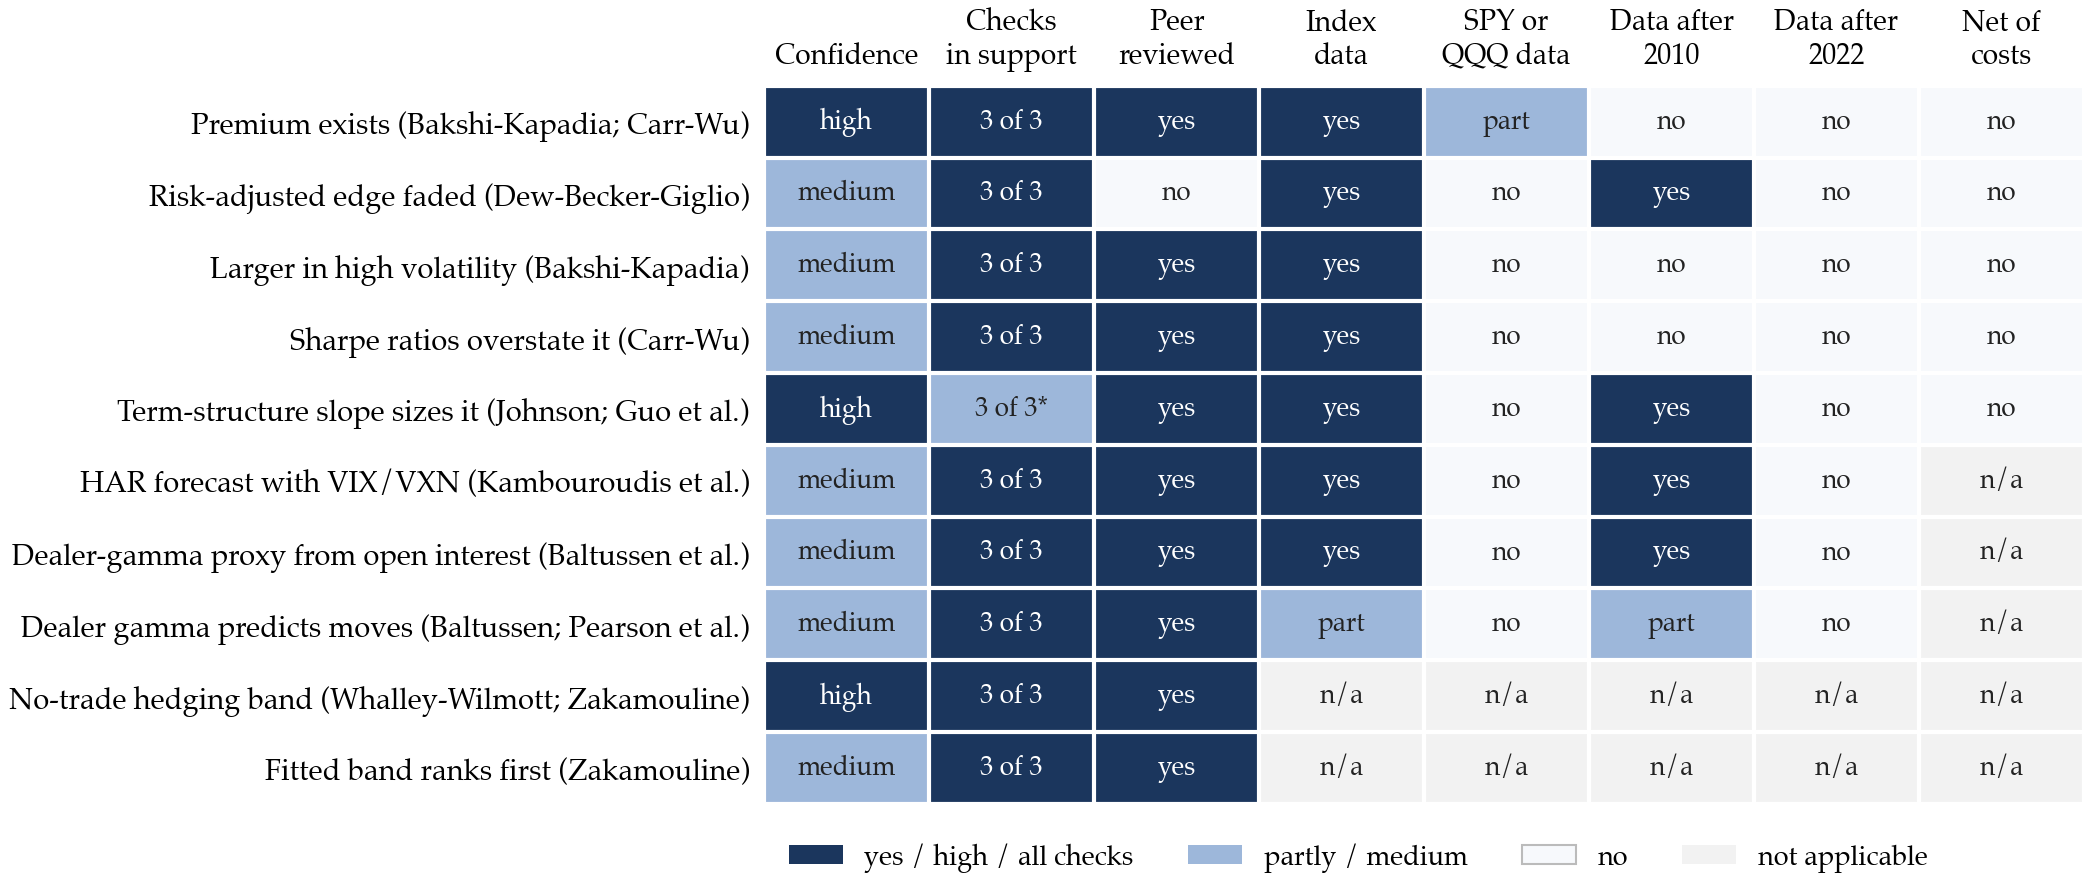
\includegraphics[width=0.9\textwidth]{figures/fig_lit_matrix.png}
\caption{What the evidence behind each finding covers, as rated in our review (29 September 2026). Columns give the confidence rating; how many of three independent checks against the primary source supported the finding (* all three on the main claim, two of three on one sub-claim); whether the source is peer reviewed; and what its data cover. ``Part'' marks a finding whose sources differ (Carr and Wu report QQQ figures beside SPX; Pearson et al.\ use single stocks and end in 2001). No finding rests on data after 2022 or on returns net of costs.}
\label{fig:litmatrix}
\qsource{Cited studies (Table~\ref{tab:evidence}); review notes, 29 September 2026; author's coding.}
\end{figure*}

\subsection{The premium exists}

Bakshi and Kapadia \cite{bakshi2003} show that buying S\&P~500 index options and delta-hedging them loses money on average, and that the mean delta-hedged gain is a vega-weighted measure of a negative volatility risk premium. Carr and Wu \cite{carrwu2009} measure the premium with synthetic variance swaps on SPX from 4~January 1996 to 28~February 2003; Table~\ref{tab:carrwu} lists the statistics our notes record from their Tables~4 and~5, and Figure~\ref{fig:litbars}(a) compares the average implied and realised volatility.

\begin{table}[tb]
\centering
\caption{Variance risk premium statistics reported by Carr and Wu \cite{carrwu2009}, 30-day horizon. SPX: 4 Jan 1996 -- 28 Feb 2003. QQQ figures are as recorded in our checking notes on the same paper; their sample period was not recorded.}
\label{tab:carrwu}
\small
\qstripes
\begin{tabular}{@{}lrr@{}}
\toprule
\qhead{Statistic} & \qhead{SPX} & \qhead{QQQ} \\
\midrule
Mean synthetic swap rate (vol pts) & 24.4 & -- \\
Mean realised volatility (vol pts) & 18.8 & -- \\
Mean $\ln(RV/SW)$, per month & $-0.594$ & $-0.257$ \\
\quad $t$-statistic & $-9.48$ & $-3.89$ \\
Mean $100\times(RV-SW)$ & $-2.279$ & $-2.940$ \\
\quad $t$-statistic & $-7.19$ & $-1.82$ \\
Std.\ dev.\ of $100\times(RV-SW)$ & 3.339 & -- \\
Skewness & $-0.597$ & -- \\
Excess kurtosis & 9.283 & -- \\
\bottomrule
\end{tabular}
\qsource{Carr and Wu (2009), Tables 4--5; review notes.}
\end{table}

Two cautions apply. The $-0.594$ is a log return and overstates the arithmetic loss to a variance-swap buyer; it should not be read as a percentage. And a delta-hedged straddle does not collect the variance-swap payoff one for one: it earns a gamma-weighted, path-dependent share of it, as equation~(\ref{eq:pnl}) shows. A later study of S\&P options over 1996--2021 by D\"orries et al., known to us only through a secondary summary \cite{dorries}, reports that short delta-hedged calls, puts and straddles kept earning premia through 2008 and the COVID-19 crash.

\begin{figure*}[t]
\centering
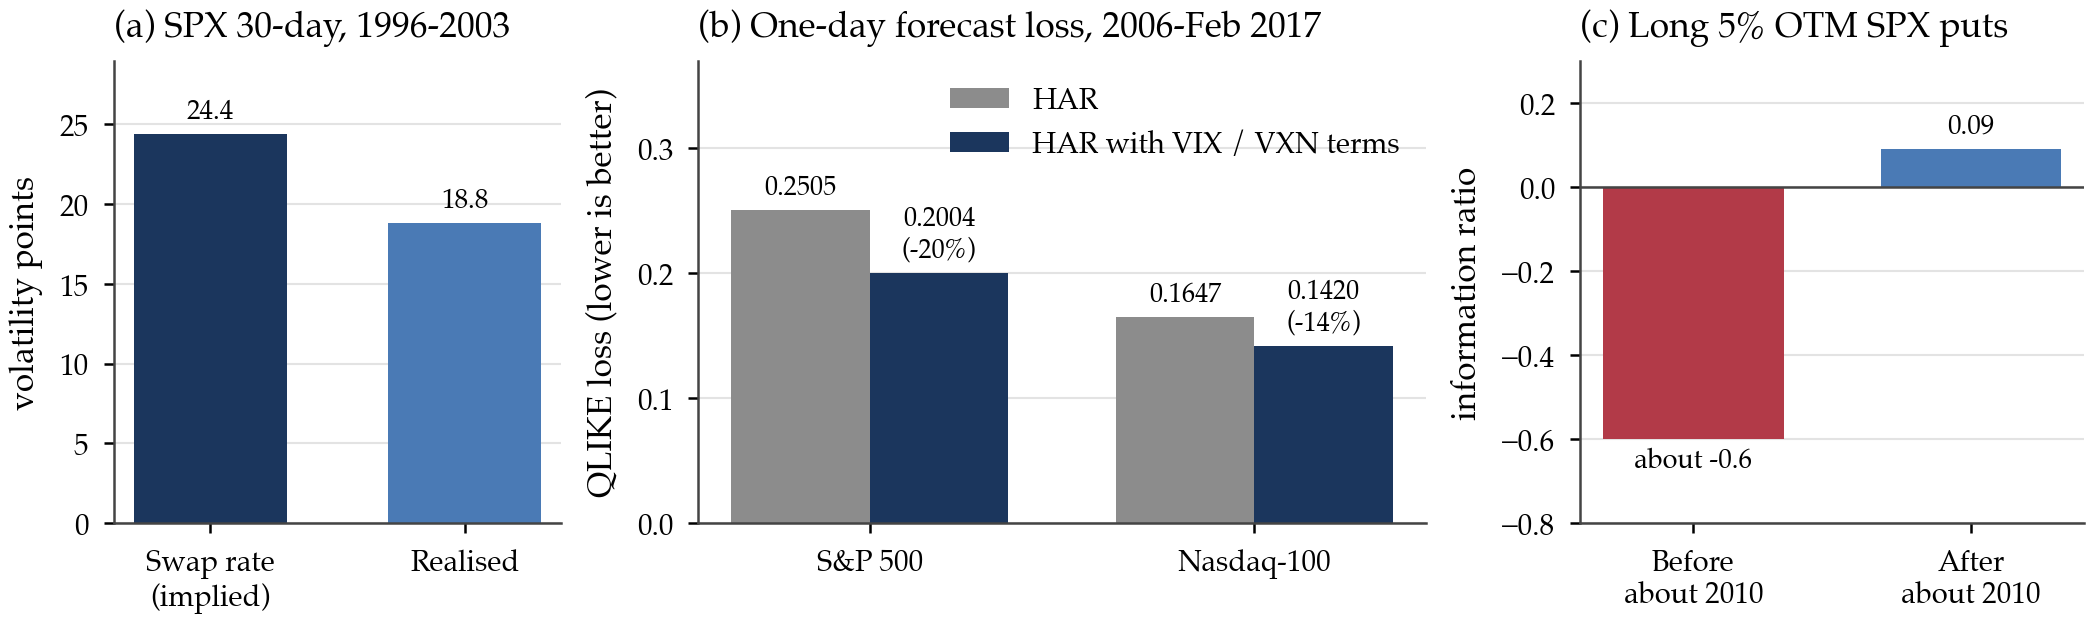
\includegraphics[width=\textwidth]{figures/fig_lit_bars.png}
\caption{Three published results, gross of costs. (a) Average 30-day synthetic variance swap rate and realised volatility on SPX, January 1996 to February 2003. (b) Out-of-sample one-day QLIKE loss of a log-HAR realised-variance model with and without VIX (S\&P~500) or VXN (Nasdaq-100) terms, rolling window 2006 to February 2017. (c) Information ratio of long 5\% out-of-the-money SPX puts before and after the break around 2010; the earlier value is reported only as about $-0.6$.}
\label{fig:litbars}
\qsource{Carr and Wu (2009), Tables 4--5; Kambouroudis et al.\ (2021), Tables 2--3; Dew-Becker and Giglio (2025, unrefereed).}
\end{figure*}

\subsection{The risk-adjusted edge has faded}

The most recent paper in the review, a Chicago Fed working paper by Dew-Becker and Giglio \cite{dewbecker2025}, finds that since about 2010 the CAPM alpha of delta-hedged SPX options has converged to zero. Besides the break in the information ratio of long out-of-the-money puts (Figure~\ref{fig:litbars}c), rolling ten-year information ratios for delta-hedged at-the-money straddles, delta-hedged 5\% out-of-the-money puts and a proxy built from realised variance minus VIX squared all rose to about zero, the straddles before the crash of March 2020. In the authors' words there is ``still a premium for variance risk'', but no larger than the CAPM beta of variance implies.

One point found in checking the paper matters for anyone quoting it: its May 2012 break date comes from a test on dealer net gamma, not on option returns; for returns it says only ``somewhere around 2010''. The paper is unrefereed, a single source and monthly SPX only, and does not cover weekly or 0DTE options, SPY or QQQ. Its implication for us is direct: a short delta-hedged SPY book should still earn a raw premium, but it should be judged against simply holding equity beta, because the premium is mostly compensation for market and crash exposure.

\begin{figure*}[t]
\centering
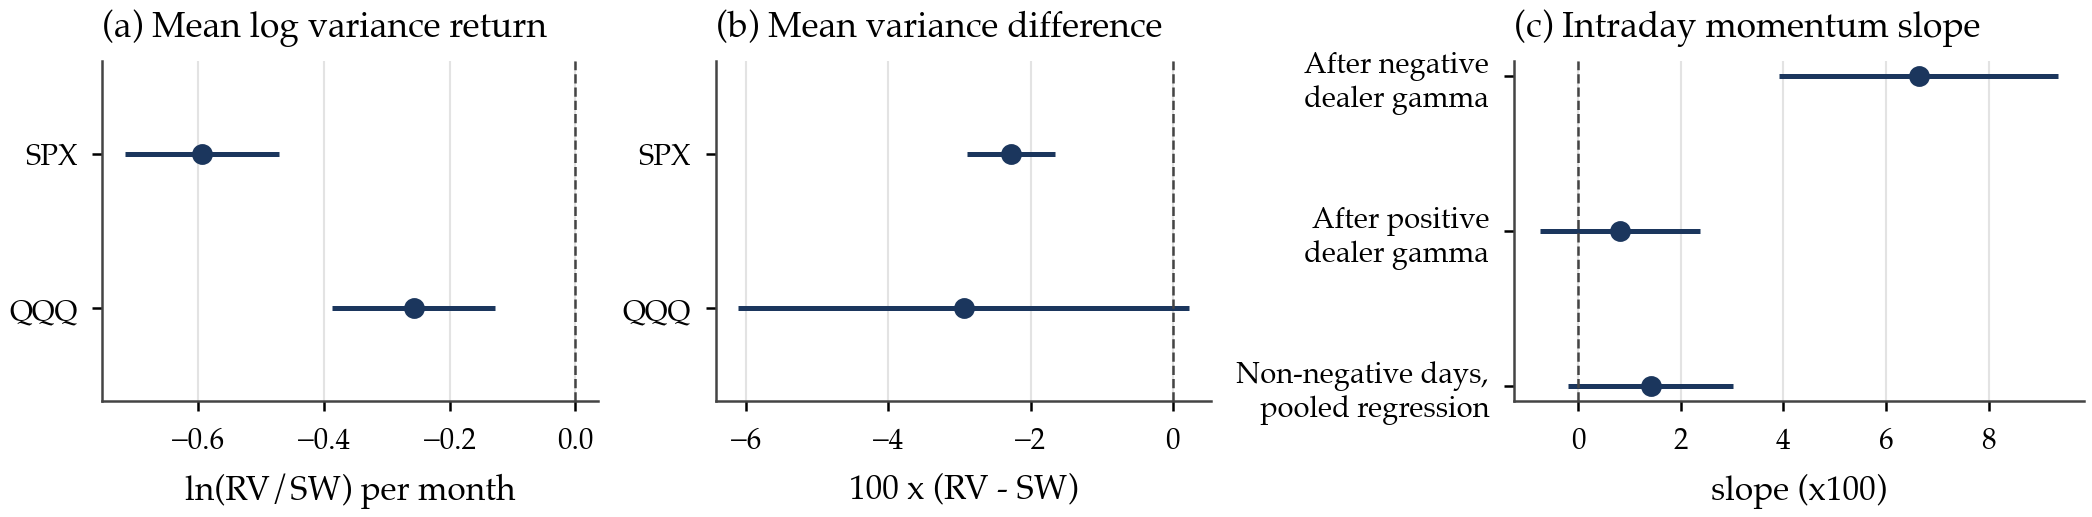
\includegraphics[width=\textwidth]{figures/fig_forest.png}
\caption{Published estimates with 95\% intervals computed as estimate $\pm1.96\times$ estimate$/t$ from the reported $t$-statistics. (a, b) Mean 30-day variance risk premium for SPX (January 1996 to February 2003) and QQQ (sample period not recorded in our notes). (c) Slope of the last-half-hour return on the rest-of-day return in S\&P~500 futures, 1996 to May 2020, after days of negative and of positive estimated dealer gamma, and on non-negative days in the pooled interaction regression.}
\label{fig:forest}
\qsource{Carr and Wu (2009); Baltussen et al.\ (2021), Tables 7--8; intervals are author's calculations.}
\end{figure*}

\subsection{The premium varies, and its tails are heavy}

Bakshi and Kapadia report that long delta-hedged options lose more when volatility is high. Huang, Schlag, Shaliastovich and Thimme \cite{huang2019} find that volatility and the volatility of volatility both predict lower delta-hedged payoffs, and a New York Fed analysis \cite{nyfed2021} reports realised-variance term premia of about 5--15\% in the 2008 crisis and the COVID-19 crash, against about 2\% on average. Part of this is mechanical, since dollar profit and loss scale with volatility, and crisis outcomes are also worse in high-volatility regimes; the finding is about average dollar losses, not risk-adjusted returns.

Short-volatility returns also look better on a Sharpe ratio than they are: raw information ratios above 3 fall to about 0.8 at most once serial dependence is accounted for (Table~\ref{tab:evidence}), and the premium is negatively skewed with fat tails (Table~\ref{tab:carrwu}). That sample ends before 2008, 2020 and the 0DTE era, and short-volatility returns collapsed in 2008--09 and in 2020. A short-gamma book should therefore be managed and judged on its tail losses, not its Sharpe ratio.

\begin{figure*}[t]
\centering
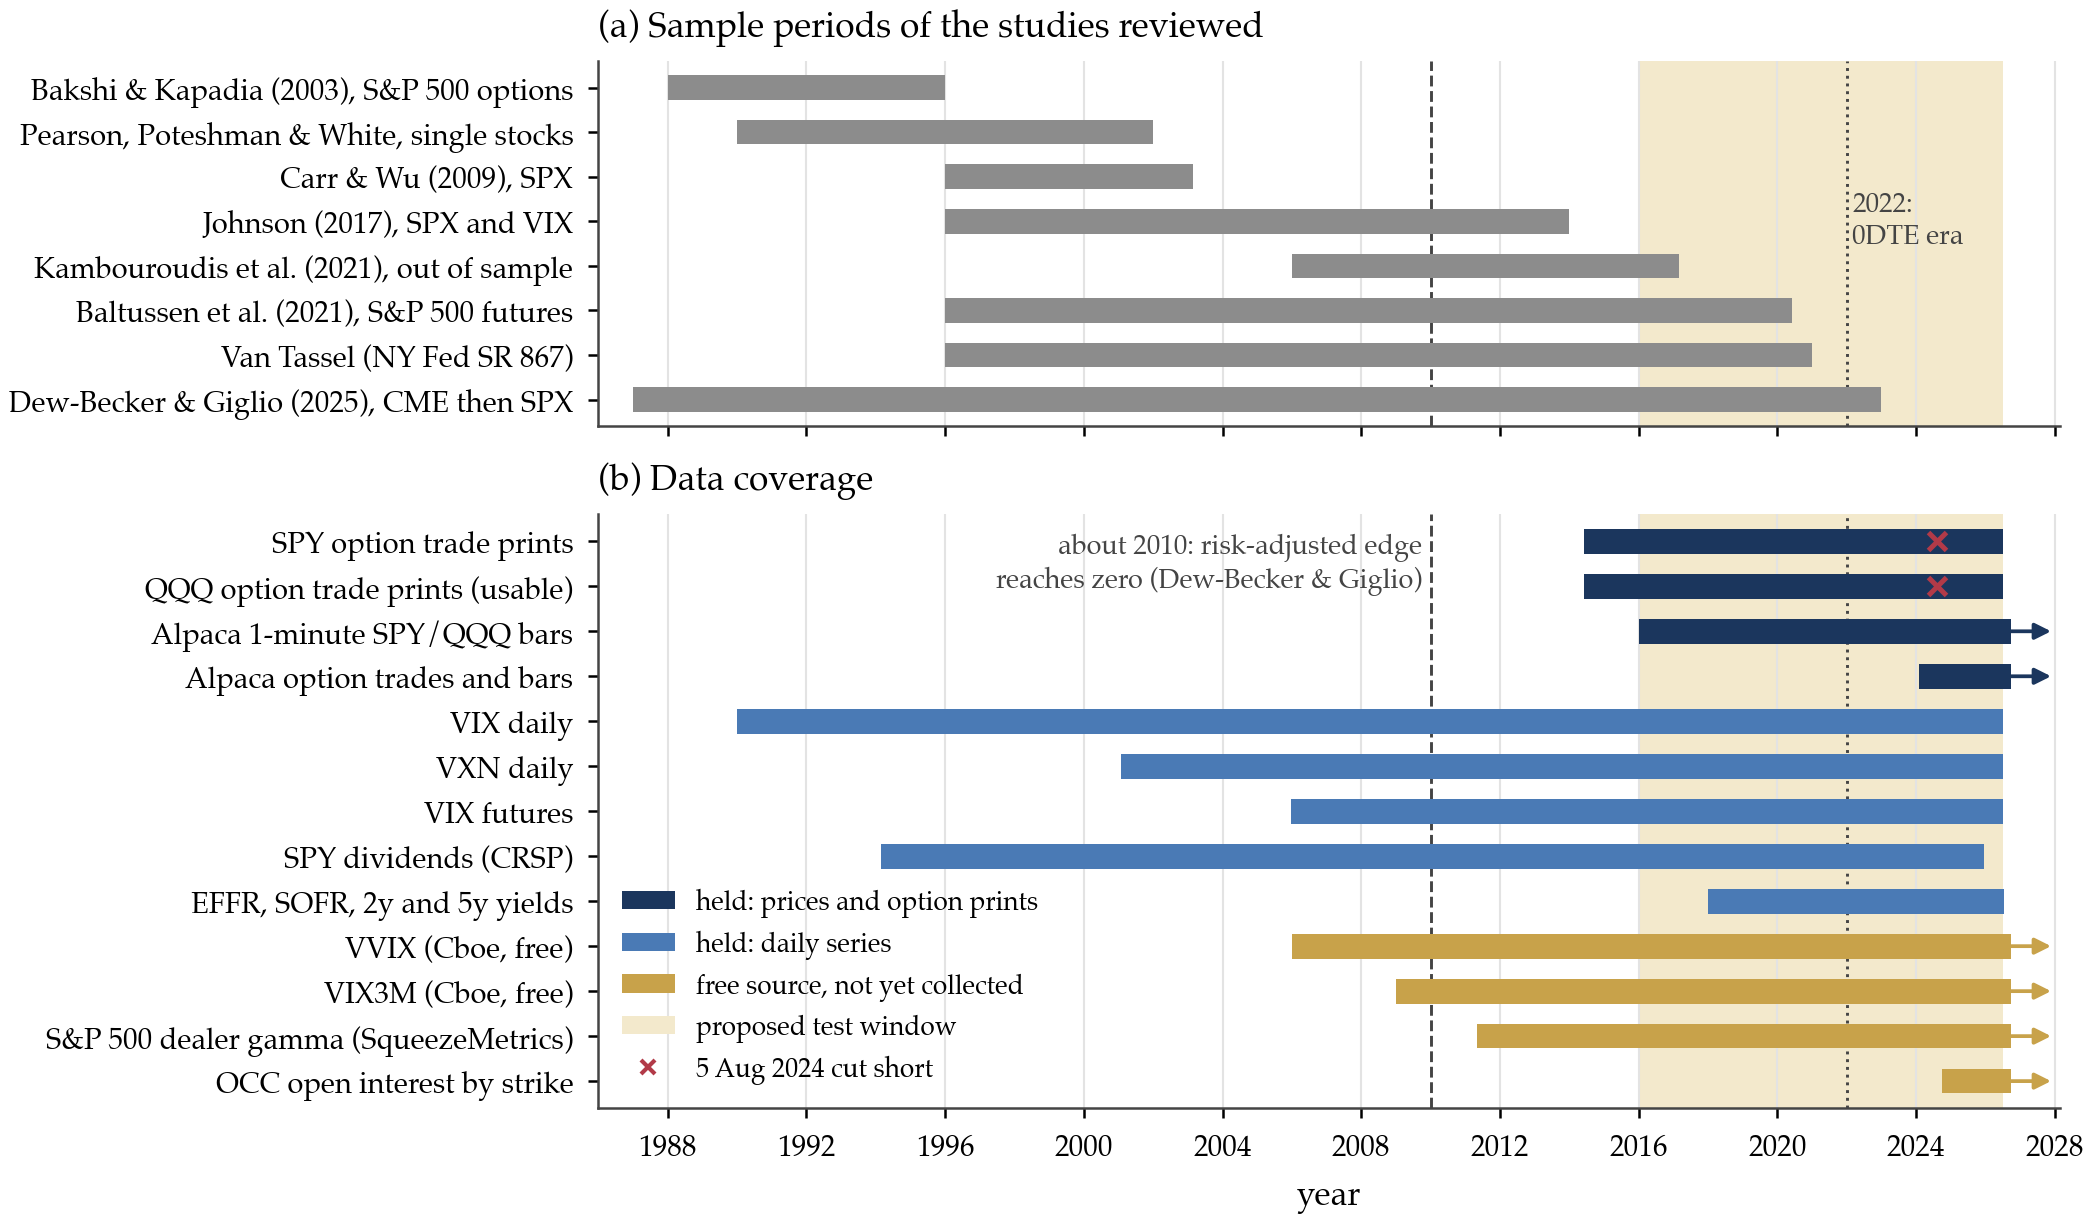
\includegraphics[width=0.86\textwidth]{figures/fig_timeline.png}
\caption{(a) Sample periods of the studies reviewed (Bakshi and Kapadia's is approximate; Guo et al.\ is omitted because its sample was not recorded). (b) Coverage of the data we hold and of free sources identified but not yet collected, as checked on 29 September 2026; arrows mark series that continue past the check, and the OCC bar shows its rolling two-year window. Crosses mark 5~August 2024, when both option-print series stop early; month-end gaps are too frequent to draw. The dashed line marks the change around 2010 reported by Dew-Becker and Giglio; the proposed test window (shaded) lies entirely after it.}
\label{fig:timeline}
\qsource{Cited studies; our option archive; Alpaca API; CRSP via WRDS; Refinitiv Datastream; Cboe; OCC; SqueezeMetrics.}
\end{figure*}

\subsection{Signals for sizing}

\textbf{Term structure.} Johnson \cite{johnson2017} shows that the slope of the VIX term structure (its second principal component) reflects the variance risk premium rather than expected changes in the VIX, rejecting the expectations hypothesis, and that it predicts returns on synthetic variance swaps, VIX futures and SPX straddles at every maturity, beyond other proxies for the premium. A steep upward slope (contango: longer-dated implied volatility above shorter-dated) predicts more negative returns to long-variance positions and so favours short gamma; a flat or inverted curve predicts relatively better long-variance returns. The quintile spreads in Table~\ref{tab:evidence} are gross of costs that the summarising source \cite{cxo} says ``may be high''. A New York Fed staff report by Van Tassel \cite{vantassel}, on 1996--2020, broadly corroborates the result. Guo, Ruan, Gehricke and Zhang \cite{guo2023} reach a similar result with the term spread of the level factor of the SPX implied-volatility curve, more strongly for straddles; the full text was not accessible, so the size of their out-of-sample fit and whether the straddles were delta-hedged are unverified. Both papers are on SPX and pre-date 0DTE options (Figure~\ref{fig:timeline}a).

\textbf{Realised-volatility forecast.} A short-gamma book earns the gap between implied and realised volatility, so it needs a forecast of the latter. The heterogeneous autoregressive (HAR) model forecasts realised variance from its own daily, weekly and monthly averages; QLIKE is a standard loss function for variance forecasts, lower being better. Kambouroudis, McMillan and Tsakou \cite{kambouroudis2021} add implied-volatility terms (VIX or VXN) to a log-HAR model of five-minute realised variance and reduce one-day-ahead loss by 20\% for the S\&P~500 and 14\% for the Nasdaq-100 (Figure~\ref{fig:litbars}b); overnight returns add further information. For the Nasdaq-100, a model with leverage and overnight terms but no implied volatility beat the plain HAR model with it, and a claim that a parsimonious implied-volatility model beats all richer ones was rejected by all three checks. Their realised variance is open to close, so it omits the overnight gap that drives close-to-close hedging profit, and the paper tests forecast accuracy over one day, not trading profit.

\textbf{A conflict between signals.} Bakshi and Kapadia find that short gamma earns more when volatility is high. Johnson finds that a flat or inverted curve, typical of high volatility, predicts better returns to long variance. One says sell more in high volatility, the other sell less. Figure~\ref{fig:signalgrid} tallies the directions the papers report, adding the dealer-gamma signal of Section~\ref{sec:gex}: the signals agree only in a steep-contango, positive-dealer-gamma state, and the inverted-curve, negative-dealer-gamma state named in the design as a candidate for long gamma is where they lean most against short gamma. The combined rule cannot be read off the papers; it has to be fitted on SPY and QQQ data.


\begin{figure}[t]
\centering
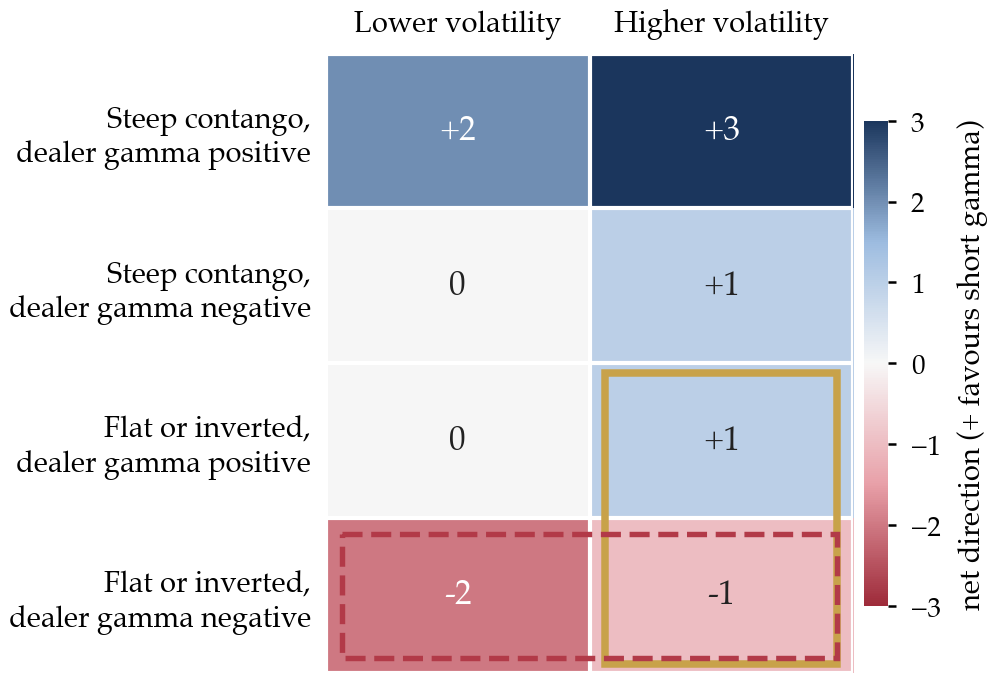
\includegraphics[width=\columnwidth]{figures/fig_signal_grid.png}
\caption{Direction of three published signals in each combination of states. Each signal is scored by the direction its paper reports: term-structure slope (steep contango $+1$, flat or inverted $-1$), volatility level (higher $+1$, lower $0$) and dealer gamma (positive $+1$, negative $-1$); a positive total favours short gamma. The totals are a tally of directions, not an estimate or a fitted rule. Gold box: states where the volatility-level and term-structure signals conflict. Dashed red box: the candidate long-gamma regime named in the design.}
\label{fig:signalgrid}
\qsource{Directions as reported by Johnson (2017), Bakshi and Kapadia (2003) and Baltussen et al.\ (2021); author's coding.}
\end{figure}

\subsection{Dealer gamma}
\label{sec:gex}

Baltussen, Da, Lammers and Martens \cite{baltussen2021} find intraday momentum in S\&P~500 futures after days of negative estimated dealer gamma (Figure~\ref{fig:forest}c). Their pooled interaction regression still shows a slope of 1.41 ($t=1.72$) on non-negative days, so the effect is not confined to negative-gamma days, and an $R^2$ of 3.58\% is weak. They note that estimated dealer gamma is positive on most days, that the proxy misses over-the-counter positions and that it only approximates end-user demand. In single stocks, Pearson, Poteshman and White \cite{pearson2006} find that higher market-maker gamma goes with smaller next-day moves, controlling for more than ten lags of absolute returns. The two agree in direction: negative dealer gamma goes with trending, larger moves and positive dealer gamma with mean reversion, which suggests an intraday overlay that leans long gamma when dealer gamma is negative and short gamma when it is positive. Neither tests SPY or QQQ, the profit of an option strategy, or the period since 2022, and the long-calls, short-puts assumption may fit SPY and QQQ worse than SPX because of heavy retail call buying there \cite{bryzgalova2023}.


\subsection{Hedging rules under costs}

With proportional costs, the theoretically preferred hedge is a band, not a clock: do nothing while the hedge ratio stays inside a no-trade region, and when it leaves, trade only back to the nearest edge, never all the way to a fully hedged position. Whalley and Wilmott \cite{whalley1997} derive the asymptotic half-width for small costs and constant absolute risk aversion:
\begin{equation}
h=\left(\frac{3\,\lambda\,e^{-r(T-t)}\,S\,\Gamma^{2}}{2\,\gamma_{\mathrm{RA}}}\right)^{1/3},
\label{eq:ww}
\end{equation}
where $\lambda$ is the proportional cost, $\Gamma$ the gamma of the whole book (for a straddle, both legs) and $\gamma_{\mathrm{RA}}$ an unobservable risk aversion that acts as a tuning setting. The band widens with cost ($\lambda^{1/3}$) and gamma ($\Gamma^{2/3}$). Two later papers confirm the formula \cite{arzel2026,imaki}.

Zakamouline \cite{zakamouline2005} centres the band on the Black--Scholes delta at an adjusted volatility, $\sigma_m^2=\sigma^2\bigl(1+h_\sigma(S^2\Gamma)^{0.15}\bigr)$, with half-width $h_w|\Gamma|^{1/2}+h_0/\bigl(S(T-t)\bigr)$ and constants tuned by simulation. In a Monte Carlo study of a short one-year at-the-money European call ($S=K=100$, $\sigma=0.25$, 1\% proportional cost, 100,000 paths), the fitted rule beat fixed-interval Black--Scholes, Leland, constant delta tolerance, asset-move tolerance, Whalley--Wilmott and Barles--Soner on both mean-against-standard-deviation and mean-against-95\%-VaR frontiers. The test is in-sample, in the same constant-volatility model with no jumps, and a later paper \cite{zakamouline2009} finds that the ranking depends on the position and on risk preferences; a claim that a simple band is enough at costs below $\lambda=0.001$ was rejected (Table~\ref{tab:refuted}), so both rules have to be tested. All of these results assume European options on a geometric Brownian motion; for American SPY and QQQ options, whose prices jump, the constants must be recalibrated by simulation. Share-hedging costs in SPY and QQQ are small (our notes put them well under one basis point, an assumption we have not measured), so the bands will be narrow.

\begin{table}[b]
\centering
\caption{Claims refuted in the review. ``Refuted'' means the wording did not survive; it does not prove the opposite.}
\label{tab:refuted}
\small
\qstripes
\begin{tabular}{@{}L{4.9cm}c@{}}
\toprule
\qhead{Claim} & \qhead{Checks in support} \\
\midrule
QQQ premium is much weaker and insignificant in level terms \cite{carrwu2009} & 1 of 3 \\
Below $\lambda=0.001$ a simple band is enough for SPY and QQQ \cite{zakamouline2005} & 1 of 3 \\
A parsimonious HAR model with implied volatility beats all richer models \cite{kambouroudis2021} & 0 of 3 \\
\bottomrule
\end{tabular}
\qsource{Review notes, 29 September 2026.}
\end{table}

\subsection{QQQ and 0DTE}

The evidence on QQQ is thin and mixed. A claim that the QQQ premium is much weaker than the SPX premium and insignificant in level terms was refuted, yet Table~\ref{tab:carrwu} and Figure~\ref{fig:forest}(a,b) show a smaller log premium for QQQ and a level premium whose 95\% interval includes zero ($t=-1.82$). A refuted claim is not proof of its opposite (Table~\ref{tab:refuted}): the size of the QQQ premium is an open question for our own data. On 0DTE options we have one second-hand data point: a study by Vilkov, as summarised by CXO Advisory and Hull Tactical \cite{vilkov}, reports that static hold-to-expiry 0DTE short straddles and condors have Sharpe ratios near zero with fat tails. We did not verify it.


%═══════════════════════════════════════════════════════
\section{Data Assessment}
\label{sec:data}

The data checks were read-only queries against our option archive, including a full scan of its timestamps for per-day trade counts, and against Alpaca's API from a paper (simulated) account; no orders were placed. Figure~\ref{fig:inventory} summarises what each input offers, and Figure~\ref{fig:timeline}(b) sets its coverage against the sample periods of the studies in Section~\ref{sec:lit}.

\begin{figure}[tb]
\centering
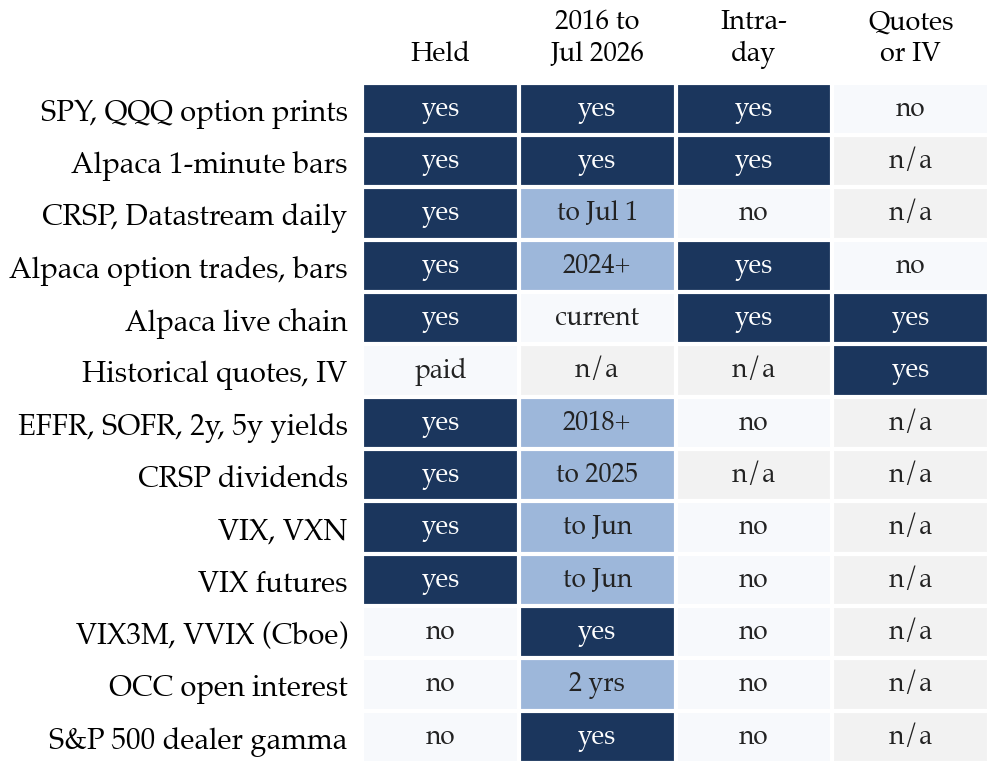
\includegraphics[width=\columnwidth]{figures/fig_inventory.png}
\caption{Attributes of each input as checked on 29 September 2026: whether we hold it, whether it covers the proposed test window from January 2016 to July 2026 (light cells state the limit), whether it is intraday, and whether it carries option quotes or implied volatilities. The only held input with quotes and implied volatilities is the live chain, which has no history. For VIX3M, VVIX and the SqueezeMetrics dealer-gamma series our notes record only the start year, so their coverage to July 2026 is assumed, not checked.}
\label{fig:inventory}
\qsource{Our option archive; Alpaca API and documentation; CRSP via WRDS; Refinitiv Datastream; Cboe; OCC; SqueezeMetrics.}
\end{figure}



\begin{table*}[t]
\centering
\caption{Defects in the option trade archive and how the design handles them. ``Measured'' items were queried on 29 Sep 2026; ``inferred'' items were not tested.}
\label{tab:defects}
\small
\qstripes
\begin{tabularx}{\textwidth}{@{}L{2.6cm}YL{1.5cm}Y@{}}
\toprule
\qhead{Defect} & \qhead{Detail} & \qhead{Evidence} & \qhead{Handling in the design} \\
\midrule
Month-end days missing & Every trading day that falls on the last calendar day of a month is absent: 98 of 98 such days through 2025, plus 31 Mar, 30 Apr and 30 Jun 2026, for SPY and QQQ alike. Every quarter-end is missing; other underlyings in the archive show the same pattern & measured & Hold positions across the gap; mark with Alpaca data where available (2024 onward) or interpolate; never drop the day's profit and loss \\
5 Aug 2024 truncated & SPY stops at 13:16 ET and QQQ at 12:52 ET, on a day of a sharp volatility spike & measured & Fill from Alpaca option trades and bars; otherwise short-volatility losses are understated \\
QQQ end & 9 Jul 2026 stops at 15:43 ET; 10 Jul 2026 absent & measured & End the QQQ window on 8 Jul 2026 \\
Exact duplicates & 3.5\% of rows on the sample day identical in every field; no sequence number separates duplicates from split fills & measured & Choose a rule (drop, or keep and flag) and test the result's sensitivity to it \\
Multi-leg prints & Condition codes 232--239, about 9\% of June 2026 prints; they print away from the market & share measured; meaning inferred & Drop before backing out implied volatility, after confirming the code meanings \\
Late and cancelled trades & A few prints with codes 202--205 & inferred & Drop \\
\bottomrule
\end{tabularx}
\qsource{Queries of our option archive, 29 September 2026.}
\end{table*}

\begin{figure*}[t]
\centering
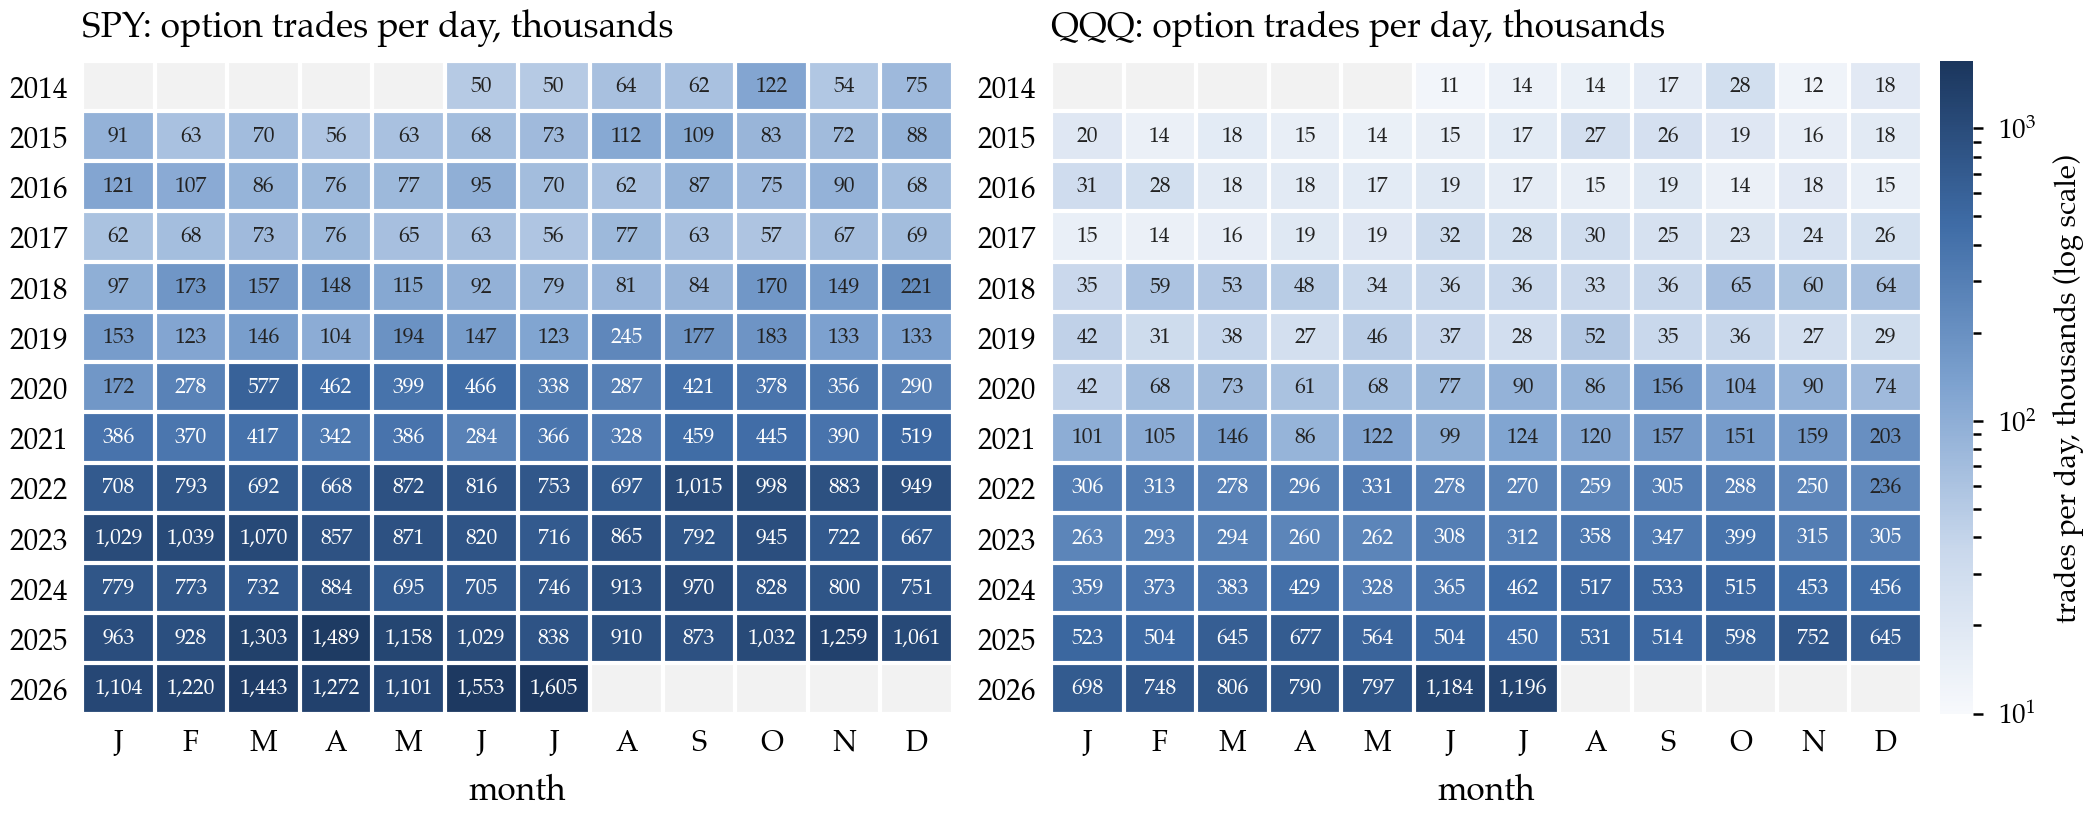
\includegraphics[width=\textwidth]{figures/fig_coverage.png}
\caption{Mean number of option trades per trading day in each month, in thousands, for SPY (left) and QQQ (right), June 2014 to July 2026, on a log colour scale. Means are over the days present in the archive: the last calendar day of each month is missing throughout (Table~\ref{tab:defects}), and July 2026 covers only the first days of the month (to 10 July for SPY and 9 July for QQQ).}
\label{fig:coverage}
\qsource{Per-day trade counts from our option archive; author's calculations.}
\end{figure*}

\subsection{The option trade archive}

We hold a tick archive of consolidated option trade prints for SPY and QQQ, one file per month, sorted by time. Each row carries a timestamp, the underlying, expiry, option type, strike, price, size, exchange code, one trade-condition code and the OCC option symbol, which matched the separately parsed contract terms on all 1,527,615 rows of the 9~July 2026 sample day. The archive holds trades only: no quotes, no national best bid and offer, no implied volatilities or greeks and no open interest (Table~\ref{tab:archive}). Figure~\ref{fig:coverage} shows how activity grew: over the days in the archive, SPY option trades per day averaged about 67,000 in 2017 and about 1.07 million in 2025, and QQQ about 23,000 and 576,000.

\begin{table}[H]
\centering
\caption{Coverage of the option trade archive, measured 29 Sep 2026.}
\label{tab:archive}
\small
\qstripes
\begin{tabular}{@{}lrr@{}}
\toprule
 & \qhead{SPY} & \qhead{QQQ} \\
\midrule
First day & 2014-06-02 & 2014-06-02 \\
Last day & 2026-07-10 & 2026-07-09\textsuperscript{a} \\
Trading days & 2,944 & 2,943 \\
Trades & 1.347\,bn & 585\,M \\
Trades on 2026-07-09 & 1,527,615 & 1,063,234 \\
\bottomrule
\rowcolor{white}\multicolumn{3}{@{}p{7.6cm}@{}}{\footnotesize \textsuperscript{a}QQQ stops at 15:43 ET on 9 July 2026; usable data end on 8 July.}
\end{tabular}
\qsource{Our option archive, per-day trade counts.}
\end{table}


On the sample day, SPY options traded about 11.8 million contracts across 5,114 distinct contracts and 36 expiries, and 70\% of SPY option trades were in options expiring that day. Weekly expiries are present from 2014; January 2022 had 12 days with a same-day expiry, when only Monday, Wednesday and Friday expiries existed; monthly expiries before 2015 are dated on a Saturday (for example, 21~June 2014).

The archive has defects that any backtest must handle (Table~\ref{tab:defects}). The most serious are the missing month-end days and the truncated 5~August 2024, a volatility spike and one of the worst days for short gamma in the sample. A backtest that skipped either would flatter a short-gamma book.


\subsection{Other data}


Table~\ref{tab:inventory} lists the other inputs and Figure~\ref{fig:inventory} summarises them. Three gaps stand out. First, the archive has no intraday SPY or QQQ price; Alpaca's one-minute consolidated bars, tested back to 4~January 2016, are the only intraday underlying we have, and they set the start of the test window. Second, no source we hold offers historical option quotes. Alpaca's historical option bars and trades start in February 2024 according to its documentation (a test contract returned bars from 18~January 2024; a 2023 contract returned nothing), and they carry no quotes either. Historical quotes and implied-volatility surfaces for earlier years are available only from paid vendors such as OptionMetrics, Cboe DataShop or ORATS. Third, the open interest a dealer-gamma estimate needs is not in the archive, and the free OCC series keeps only a rolling two-year window, so it must be archived daily from now on.

\begin{table*}[t]
\centering
\caption{Inputs other than the option prints: what we hold, what can be collected free, and what is missing, as checked on 29 Sep 2026.}
\label{tab:inventory}
\small
\qstripes
\begin{tabularx}{\textwidth}{@{}L{2.7cm}L{3.0cm}L{4.6cm}Y@{}}
\toprule
\qhead{Need} & \qhead{Source} & \qhead{Coverage} & \qhead{Status and limits} \\
\midrule
Intraday SPY, QQQ & Alpaca 1-minute bars & From 4 Jan 2016 & Held; live hedging would use the IEX feed or delayed data \\
Daily SPY, QQQ & CRSP via WRDS; Datastream & To 31 Dec 2025; to 1 Jul 2026 & Held; daily only \\
Option trades and bars & Alpaca & From Feb 2024 & Held; patches 5 Aug 2024 and recent month-ends \\
Historical option quotes & None & -- & Missing; paid vendors only \\
Live chain with IV, greeks & Alpaca indicative feed & Current only & Held; OPRA quotes need a signed agreement \\
Interest rates & EFFR, SOFR, 2y, 5y yields & 2018 to mid-July 2026 & Held; H.15 curve stale after Feb 2025 \\
Dividends & CRSP distributions & SPY: 128 payments to 19 Dec 2025; QQQ: 81 to 22 Dec 2025 & Held; 2026 ex-dates from Nasdaq calendar \\
VIX, VXN & Cboe & From 1990 and Feb 2001, to 30 Jun 2026 & Held \\
VIX futures & Refinitiv Datastream & 245 contracts, 22 Dec 2005 -- 30 Jun 2026 & Held \\
VIX9D, VIX3M, VVIX & Cboe, free daily files & VIX3M from 2009, VVIX from 2006 & Not yet collected \\
Open interest by strike & OCC & Rolling two-year window & Not yet collected; archive daily \\
S\&P~500 dealer gamma & SqueezeMetrics & Daily from May 2011 & Not yet collected; vendor model, no service agreement \\
OptionMetrics, TAQ & -- & -- & Not held beyond small samples \\
\bottomrule
\end{tabularx}
\qsource{Alpaca API and documentation; CRSP via WRDS; Refinitiv Datastream; Cboe; OCC; SqueezeMetrics.}
\end{table*}

\subsection{Execution venue}

\begin{figure*}[t]
\centering
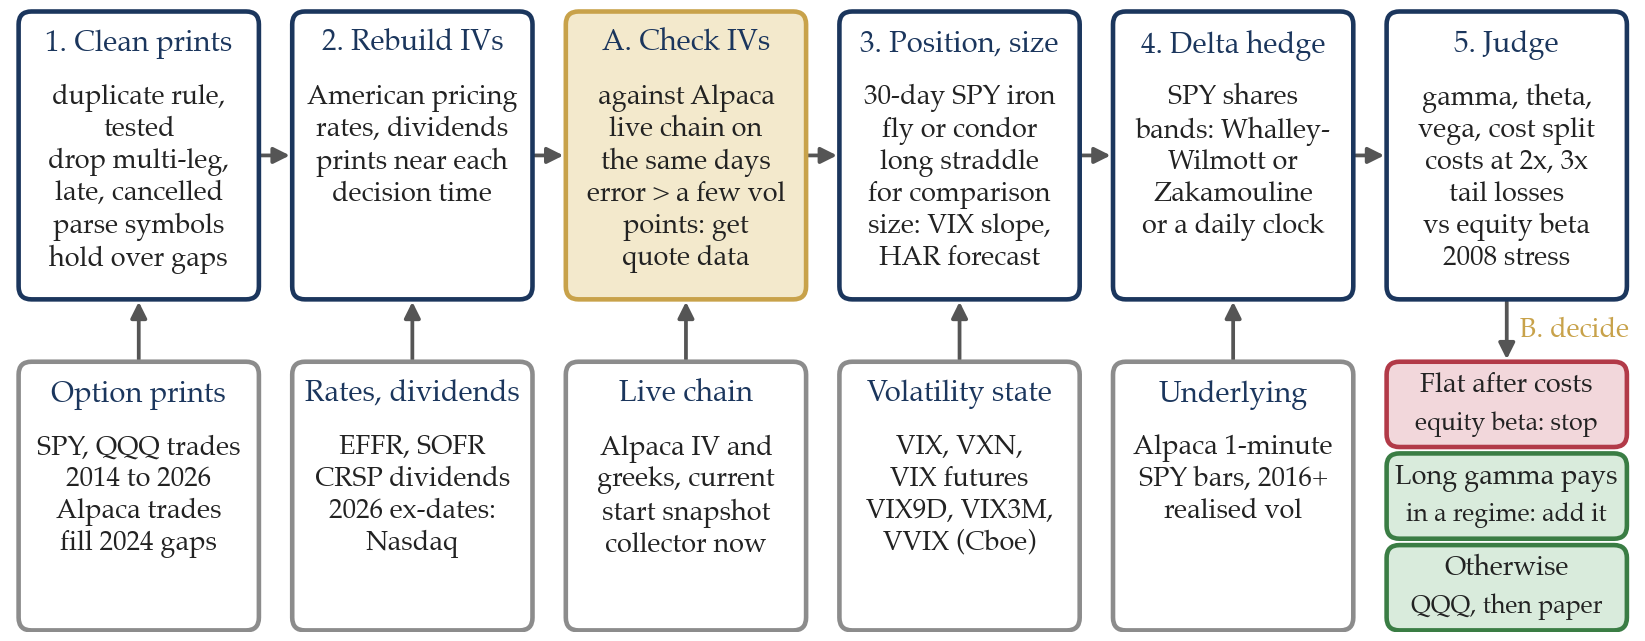
\includegraphics[width=\textwidth]{figures/fig_design.png}
\caption{The proposed test. Top row: the build sequence. Bottom row: the data feeding each step. Gate A decides whether volatilities rebuilt from trade prints are good enough to drive the signals; Gate B applies the decision rules of Table~\ref{tab:judge}. Nothing in this figure has been built or run.}
\label{fig:design}
\qsource{Design notes, September 2026.}
\end{figure*}


Alpaca was checked from a paper account with options trading level 3. Its documentation \cite{alpaca} sets four constraints. Multi-leg orders carry up to four legs and every leg must be covered within the same order, so naked short straddles and strangles cannot be sent and the short-gamma position must be an iron fly or condor. A multi-leg order cannot include a stock leg, so each delta hedge is a separate share order. Leg ratios must be in lowest terms, and rolling a short contract or a calendar can be rejected because it creates an uncovered short leg inside one order. Margin is the maximum theoretical loss across strikes for each expiry, taking the largest across expiries. Paper fills do not model real slippage, so paper trading tests the order path, not costs. The indicative feed does return implied volatilities and greeks, although its quotes are modified and its trades delayed by 15 minutes: on the check date, a SPY call struck at 755 and expiring 30~October 2026 showed an implied volatility of 14.9\%, a delta of 0.65 and a gamma of 0.011.

%═══════════════════════════════════════════════════════
\section{Proposed Test}
\label{sec:design}

The first test is the version our data support best: a 30-day SPY iron fly or condor on real prices from January 2016, when the one-minute bars start, to July 2026, when the archive ends; hedged daily and then under band rules; and sized by regime, with a long straddle as the comparison case. Figure~\ref{fig:design} shows the sequence of steps, the data that feed each, and the two points at which the work stops or changes course.



\subsection{Cleaning and implied volatilities}

The panel is cleaned first: duplicates under a stated rule whose effect is tested, multi-leg and late or cancelled prints dropped once their codes are confirmed, OCC symbols parsed and the Saturday-dated expiries handled. Implied volatilities then come from an American pricing model with overnight rates and the CRSP dividend history, with 2026 ex-dates from the Nasdaq calendar; treating SPY options as European or ignoring dividends is one of the errors the design is meant to avoid, as is marking illiquid strikes at a stale last trade.

These volatilities are the weakest link, so they are checked before anything depends on them. On days where both exist, volatilities from trade prints are compared with those in Alpaca's live chain. If the errors exceed a few volatility points, the signals cannot be trusted at the precision a premium of a few points requires, and the work turns to quote data: paid surfaces, or our own archive of chain snapshots. That archive should start now whatever the backtest finds: SPY and QQQ chain snapshots (quotes, implied volatility, greeks, open interest) saved every 15 to 30 minutes would within a few months give a quote history against which to check both the cost assumptions and the print-based volatilities.

\subsection{Positions, sizing and hedging}

The base run is an unconditional short iron fly with a daily hedge, so that the raw premium on SPY is measured before any signal is added. Regime sizing then scales the position between full size and flat, with realised volatility built from one-minute bars both open to close and close to close, since the overnight gap drives close-to-close hedging profit. The sizing rule has to resolve the signal conflict of Section~\ref{sec:lit}, which means fitting it on our data. The three hedging rules are then compared on the same positions. The choice of a 30-day structure follows from the data: in our assessment, which is not yet measured, the error from missing bid and ask prices is small relative to the profit and loss of a 30-day position hedged daily, workable with conservative cost assumptions for weekly options hedged intraday, and fatal for 0DTE trading, where the spread is most of the edge.

\subsection{Stress test}

The real-price window contains no episode like 2008, so the design adds a synthetic 2008 run with options priced from the VIX. Because the VIX sits a few volatility points above at-the-money implied volatility, that gap is calibrated on the real-price years before it is applied.

\subsection{How the test will be judged}

The test is judged against holding equity beta, not against zero, because the premium is mostly payment for crash risk; and on tail losses (the worst day, the worst month and the maximum drawdown) rather than the Sharpe ratio. Costs enter as an effective spread estimated from the bounce of successive trade prints, stressed at two and three times, because there are no quotes from which to measure the spread directly. The daily attribution into gamma, theta, vega and cost separates a premium from luck. Table~\ref{tab:judge} states in advance what each outcome would mean. QQQ comes second, once the SPY results hold, with its own estimate of the premium rather than one carried over from SPX, and a strategy that passes would be traded on Alpaca's paper account before any capital is committed.

\begin{table}[tb]
\centering
\caption{Decision rules set before the test is run.}
\label{tab:judge}
\small
\qstripes
\begin{tabular}{@{}L{3.6cm}L{3.8cm}@{}}
\toprule
\qhead{If the test finds\ldots} & \qhead{then\ldots} \\
\midrule
Print-based implied volatilities err by more than a few volatility points & the signals cannot be trusted; obtain quote data first \\
Short gamma is flat after costs, as the post-2010 literature implies & the strategy is equity beta with extra steps; stop \\
A regime (for example, an inverted term structure with negative dealer gamma) in which long gamma is positive after costs & add a long-gamma leg in that regime \\
A positive, regime-sized short-gamma result on SPY & repeat on QQQ, then trade it on paper before any capital \\
\bottomrule
\end{tabular}
\qsource{Design notes; the rules were written before any test.}
\end{table}

%═══════════════════════════════════════════════════════
\qneed{9\baselineskip}
\section{Open Questions and Limitations}
\label{sec:open}

\subsection{Questions the test must answer}

No verified evidence covers four questions that decide whether the strategy is viable.

\textbf{Implied volatility from trade prints.} Can daily SPY and QQQ implied-volatility surfaces be rebuilt from trades alone, despite stale and odd-lot prints, bid--ask bounce, early exercise and dividends, accurately enough that the errors do not swamp a premium of a few volatility points?

\textbf{Costs.} What are the all-in costs of two- to four-leg SPY and QQQ orders through Alpaca, by days to expiry and moneyness? With the risk-adjusted premium near zero since 2010, is short delta-hedged SPY gamma still positive after costs, and does QQQ carry a meaningful premium at all?

\textbf{Long gamma.} Do the term-structure and HAR signals ever identify states in which long delta-hedged gamma pays after costs, or do they only scale short gamma between full size and flat? How does the tension between high volatility and an inverted curve resolve on SPY and QQQ?

\textbf{Dealer gamma.} Can a usable SPY and QQQ dealer-gamma series be built from OCC open interest and a sign assumption, and does dealer gamma still predict intraday momentum and volatility in the 0DTE era since 2022?

\subsection{Limitations}

\textbf{Of the evidence.} No claim survived verification on transaction costs and slippage for SPY and QQQ options or multi-leg orders, on backtesting with trade-only data, on early exercise and dividends, on sizing, stop rules or vega limits beyond tail statistics, or on 0DTE options; equation~(\ref{eq:pnl}) was not verified separately. Nearly all the evidence is on SPX, and QQQ is the least supported. Most samples end between 2001 and 2022 (Figure~\ref{fig:timeline}): the main premium sample in 2003, the term-structure sample in 2013, the forecasting sample in 2017 and the dealer-gamma sample in 2020. The strongest recent paper is unrefereed. Every figure is gross of costs at mid quotes and must be re-derived net of realistic spreads, and the band rules come from single European options under geometric Brownian motion and must be recalibrated on SPY and QQQ paths with jumps and stochastic volatility.

\textbf{Of the design.} The whole real-price window lies after 2010, when the most recent evidence finds no risk-adjusted edge, so a flat result would be no surprise; the decision rules allow for it. The design does not yet fix how the window will be split in time or which volatility regimes results will be reported in; both should be set before the run, so that a result driven by one year or one episode is visible. The cost estimate from print bounce and the synthetic 2008 run both rest on calibrations not yet tested.

%═══════════════════════════════════════════════════════
\section{Conclusion}
\label{sec:conclusion}

The literature supports a narrow conclusion. Selling delta-hedged index options has earned a premium, the premium has heavy left tails that Sharpe ratios hide, and the one recent study of its risk-adjusted value finds it has been about zero since around 2010. The slope of the volatility term structure is the best-supported guide to how much of it to hold, and there is no verified case for switching to long gamma. Our data can support a real-price test on SPY from 2016 to July 2026, provided the volatilities rebuilt from trade prints pass a check against live quotes and the archive's gaps are handled rather than skipped. On the evidence, the most likely outcomes are a small premium that is largely market exposure, or a finding that we need quote data first; either is worth knowing before any capital is committed.

\section*{Status}

This design has not yet been run. No code has been written for it, and no figure in this paper is a backtest result of ours: every return statistic is quoted from the cited literature. The data checks in Section~\ref{sec:data} were run on 29~September 2026. The option archive and the licensed data (CRSP via WRDS, Refinitiv Datastream) are not distributed.

%═══════════════════════════════════════════════════════
\begin{thebibliography}{99}
\footnotesize

\bibitem{ahmad2005}
Ahmad and Wilmott.
\newblock ``Which free lunch would you like today, Sir?''
\newblock \textit{Wilmott Magazine}, November 2005.

\bibitem{alpaca}
Alpaca.
\newblock ``Historical option data'' and ``Options Level 3 trading.''
\newblock Developer documentation, accessed September 2026. \url{https://docs.alpaca.markets}

\bibitem{arzel2026}
Arzel and Lehdili.
\newblock ``Bridging stochastic control and deep hedging: Structural priors for no-transaction band networks.''
\newblock arXiv:2603.29994, 2026 (Eq.~40 restates the Whalley--Wilmott half-width).

\bibitem{bakshi2003}
Bakshi and Kapadia.
\newblock ``Delta-hedged gains and the negative market volatility risk premium.''
\newblock \textit{Review of Financial Studies}, 16(2):527--566, 2003.

\bibitem{baltussen2021}
Baltussen, Da, Lammers and Martens.
\newblock ``Hedging demand and market intraday momentum.''
\newblock \textit{Journal of Financial Economics}, 142(1):377--403, 2021.

\bibitem{bryzgalova2023}
Bryzgalova, Pavlova and Sikorskaya.
\newblock ``Retail trading in options and the rise of the big three wholesalers.''
\newblock \textit{Journal of Finance}, 78(6):3465--3514, 2023.

\bibitem{carrwu2009}
Carr and Wu.
\newblock ``Variance risk premiums.''
\newblock \textit{Review of Financial Studies}, 22(3):1311--1341, 2009.

\bibitem{cxo}
CXO Advisory Group.
\newblock Summary of Johnson (2017), ``Risk premia and the VIX term structure.''

\bibitem{dewbecker2025}
Dew-Becker and Giglio.
\newblock ``The decline of the variance risk premium: Evidence from traded and synthetic options.''
\newblock Federal Reserve Bank of Chicago Working Paper 2025-17, September 2025 (not peer reviewed).

\bibitem{dorries}
D\"orries, Korn and Power.
\newblock ``How should the long-term investor harvest variance risk premiums?''
\newblock CFR Working Paper 23-06, University of Cologne. Results cited here are from a Quantpedia summary.

\bibitem{goetzmann2002}
Goetzmann, Ingersoll, Spiegel and Welch.
\newblock ``Sharpening Sharpe ratios.''
\newblock NBER Working Paper 9116, 2002. As cited by Carr and Wu (2009).

\bibitem{guo2023}
Guo, Ruan, Gehricke and Zhang.
\newblock ``Term spreads of implied volatility smirk and variance risk premium.''
\newblock \textit{Journal of Futures Markets}, 43(7):829--857, 2023 (full text not accessed).

\bibitem{huang2019}
Huang, Schlag, Shaliastovich and Thimme.
\newblock ``Volatility-of-volatility risk.''
\newblock \textit{Journal of Financial and Quantitative Analysis}, 54(6):2423--2452, 2019.

\bibitem{imaki}
Imaki, Imajo, Ito, Minami and Nakagawa.
\newblock ``No-transaction band network: A neural network architecture for efficient deep hedging.''
\newblock arXiv:2103.01775, 2021.

\bibitem{johnson2017}
Johnson.
\newblock ``Risk premia and the VIX term structure.''
\newblock \textit{Journal of Financial and Quantitative Analysis}, 52(6):2461--2490, 2017.

\bibitem{kambouroudis2021}
Kambouroudis, McMillan and Tsakou.
\newblock ``Forecasting realized volatility: The role of implied volatility, leverage effect, overnight returns, and volatility of realized volatility.''
\newblock \textit{Journal of Futures Markets}, 41(10):1618--1639, 2021.

\bibitem{nyfed2021}
Smith and Van Tassel.
\newblock ``Equity volatility term premia.''
\newblock \textit{Liberty Street Economics}, Federal Reserve Bank of New York, 3 February 2021.

\bibitem{pearson2006}
Pearson, Poteshman and White.
\newblock ``Does option trading have a pervasive impact on underlying stock prices?''
\newblock Working paper; published with Ni as first author in \textit{Review of Financial Studies}, 34(4):1952--1986, 2021.

\bibitem{vantassel}
Van Tassel.
\newblock ``Relative pricing and risk premia in equity volatility markets.''
\newblock Federal Reserve Bank of New York Staff Report No.~867, 2018.

\bibitem{vilkov}
Vilkov.
\newblock ``0DTE trading rules.''
\newblock SSRN Working Paper 4641356, 2023. Results cited here are from summaries by CXO Advisory Group and Hull Tactical; the original was not read.

\bibitem{whalley1997}
Whalley and Wilmott.
\newblock ``An asymptotic analysis of an optimal hedging model for option pricing with transaction costs.''
\newblock \textit{Mathematical Finance}, 7(3):307--324, 1997.

\bibitem{zakamouline2005}
Zakamouline.
\newblock ``Efficient analytic approximation of the optimal hedging strategy for a European call option with transaction costs.''
\newblock \textit{Quantitative Finance}, 6(5):435--445, 2006 (presented at the European Financial Management Association meeting, Milan, 2005).

\bibitem{zakamouline2009}
Zakamouline.
\newblock ``The best hedging strategy in the presence of transaction costs.''
\newblock \textit{International Journal of Theoretical and Applied Finance}, 12(6):833--860, 2009.

\end{thebibliography}

\end{document}
